\documentclass{article}
\usepackage{graphicx} 
\usepackage[dutch]{babel}
\usepackage{logicproof}

\usetikzlibrary{automata,positioning}

\usepackage[all]{xy}

\usepackage{tikz}
\usetikzlibrary{cd}
 
\usepackage{mathtools,halloweenmath}
\begin{document}
	\sffamily
	\begin{titlepage}
		\centering
		\vfill
		{\bfseries\Huge
			Verslag Tinlab Advanced Algorithms \\
			\vskip2cm
		}
		{\bfseries\Large
			T. Ravensbergen\\ 
			G. Bartes\\
			K. G. Razmjou\\
		}
		{
			\bfseries\normalsize
			69\\
			\vskip1cm
			\today\\
		}    
		\vfill
		
\includegraphics[width=4cm]{logohr.png} % also works with logo.pdf
		\vfill
		\vfill
	\end{titlepage}
\newpage
\chapter{List of Authors}


Provide contact information of persons who have contributed considerably in collection, exploration and/or writing the literature.
The author list may be ordered alphabetically or on the basis of involvement. The name of the author who has done most of the research work, that is, collection and writing of literature, and so on, appears first on the list. Authors listed between first and last author have substantial contribution in completion of the research. Usually, it is assumed that the last author named on the list organized the review plan and proposed the original idea.


\newpage
\chapter{Managementsamenvatting}
samenvatting, introductie, omschrijving, ontwerp, testopstelling en resultaten, conclusie 

Introduction
Which is the main theme of the study?What is already known about the theme?What is not yet known about the theme?What are the objectives of the research?Are the objectives clear and well defined?Organize  Introduction  in  a  way  that  the  sequence  of  ideas  is  evident. The text should be informative, concise, and encourage the continuity of reading. 

Methods
What is the design of the study? Which is the population of the study (including studied groups and socio-demographic characterization)?Which were the inclusion and exclusion criteria considered?Which were the materials and procedures used?How was the data analysis conducted (including studied variables and statistical tests used to answer each objective, level of significance adopted, and possible transformations applied to the data)?Which were ethical procedures conducted?Write the Methods section in a way that allows its reproduction by other researchers. 

Results
Which  results  should  be  presented  to  answer  each  objective  of  the study?What  is  the  most  appropriate  way  to  summarize  each  result,  emphasizing the main findings (text, tables and/or figures)?Which statistical results should be presented to provide credibility to the findings?Besides  numerical  data,  present  a  brief  conclusion  about  the  results, in order to summarize the main findings. Data should not be discussed in this section.

Discussion
Which are the main answers to the objectives of the study?How are the findings related to those of previous studies found in literature? How do they answer the gap in knowledge evidenced in the Introduction?What are the clinical and scientific implications of the study?What are the limitations of the study?What are the perspectives of future studies on the theme, based on the results and limitations of the present study?The  authors  should  try  to  position  themselves  in  relation  to  the  findings discussed, for this is what determines the contribution of the study to Science.

Conclusion
What specific results answer to the objectives of the study?What is the novelty found in the results?Write  the  Conclusion  in  one  concise  and  accurate  paragraph,  sticking to the answer. 



	\newpage
	\tableofcontents
	
	\newpage
	\section{Inleiding}
	In deze case study wordt %insert inleiding hier
	
		\subsection{Algemeen}
	
	
	
	\subsection{Achtergrond}
	
	\subsubsection{Formal specification}
	
	\subsubsection{Modelling}
	
	\subsubsection{Formal verification}
	Formal verification is een proces warin wordt bevestigd dat het bestudeerde systeem voldoet aan de requirements of specificaties. Formele verificatie kan worden uitgevoerd door middel van simulatie, propositielogica en model checking. Deze technieken worden ondeer andere gebruikt voor het test van een systeem op safety,liveness, deadlock freeness en reachability requirements.
	
	\subsubsection{Counterexample analysis}
	Er is onderzoek gedaan naar verschillende sluizen en de bediening hiervan. 
	Een alternatief is voorgesteld om aan te tonen dat de implementatie van de sluis voldoet aan het vier-variabelen model.
	
	\subsection{Statistical model checking}
	Dit gaat in het algemeen over ...
	https://project.inria.fr/plasma-lab/statistical-model-checking/
	https://ris.utwente.nl/ws/portalfiles/portal/28200786/A_statistical_model_checker.pdf
	https://dl.acm.org/doi/pdf/10.1145/3158668
	https://dl.acm.org/doi/10.1145/3158668
	https://www-verimag.imag.fr/Statistical-Model-Checking-814.html?lang=en#:~:text=Statistical%20Model%20Checking%20(SMC)%20is,from%20state%20space%20explosion%20issues.
	https://www.comp.nus.edu.sg/~cs5270/Notes/chapt6a.pdf
	\subsection{Het vier variabelen model}
	Dit gaat in het specifiek  over  dit model
	
	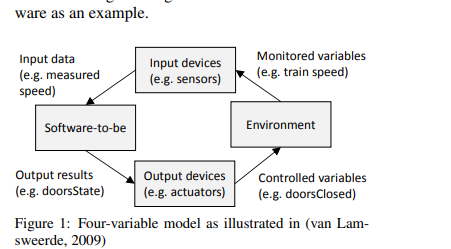
\includegraphics[width=4cm]{4varmodel.png} % also works with logo.pdf
	\subsubsection{Monitored variabelen}
	Monitored: De staatvariabele kan de waterhoogte in de sluis zijn. Dit is een interne variabele die de huidige toestand van de sluis weergeeft. Het wordt beïnvloed door de ingangsvariabele (positie van het schip) en de besturingsvariabele (bediening van de sluisdeuren en sluiskleppen).
	\subsubsection{Controlled variabelen}
		Controlled: De besturingsvariabele kan de positie van de sluisdeuren en sluiskleppen zijn. Dit zijn de bedieningselementen die worden aangepast om het schutproces te regelen. Ze kunnen open of gesloten zijn, afhankelijk van de toestand van de sluis en het schip.
	\subsubsection{Input variabelen}
	Ingangsvariabele: De ingangsvariabele kan de positie van een schip zijn, bijvoorbeeld de hoogte van de waterlijn van het schip ten opzichte van de waterhoogte in de aankomende sluis. Deze variabele beïnvloedt hoe de sluis reageert en welke acties worden ondernomen.
	\subsubsection{Output variabelen}
	Uitgangsvariabele: De uitgangsvariabele kan de positie van het schip zijn nadat het de sluis heeft verlaten. Dit kan de hoogte van de waterlijn van het schip zijn ten opzichte van de waterhoogte in de volgende waterweg. Het geeft het resultaat weer van het schutproces in de sluis.

	
	
	
	
	\subsection{Counterexamples}
	Het sluizenpartk is in beheer van Rijkswaterstaat. Onderzoek naar de werking en bediening van  sluizen
	heeft een fucntionele beschrijving van de bediening vn schutsluizen opgeleverd. Een formele omschrijving van de gevisualiseerde schutsluis is alls volgd:
	Schip komt aanvaren
	Schip meld zijn aan
	Sluisdeuren gaan open
	Stoplichten gaan op groen
	Schip vaart in de sluiskolk.
	Sluisdeuren gaan dicht en stoplicht op rood.
	De sluis start het nivelleerproces.
	De sluisdeuren  gaan open en stoplicht gaat op groen.
	Het schip kan de andere kant uitvaren
	De sluisdeuren sluiten en stoplicht gaat op rood.

 
	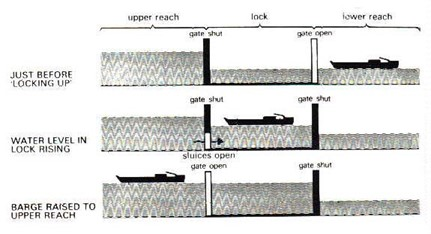
\includegraphics[width=8cm]{sluismodel.jpg} % also works with logo.pdf
	
 Het stroomschema van de richtlijn vaarwegen is een geschikte weergave volgens het 4-variabelen model.
 De input variabelen
 
 De output variabelen
 
 De monitored variabelen
 
 De controlled variabelen
 
 
		Hieronder een voorbeeld van de werking van en sluismodel volgens de richtlijn vaarwegen.
	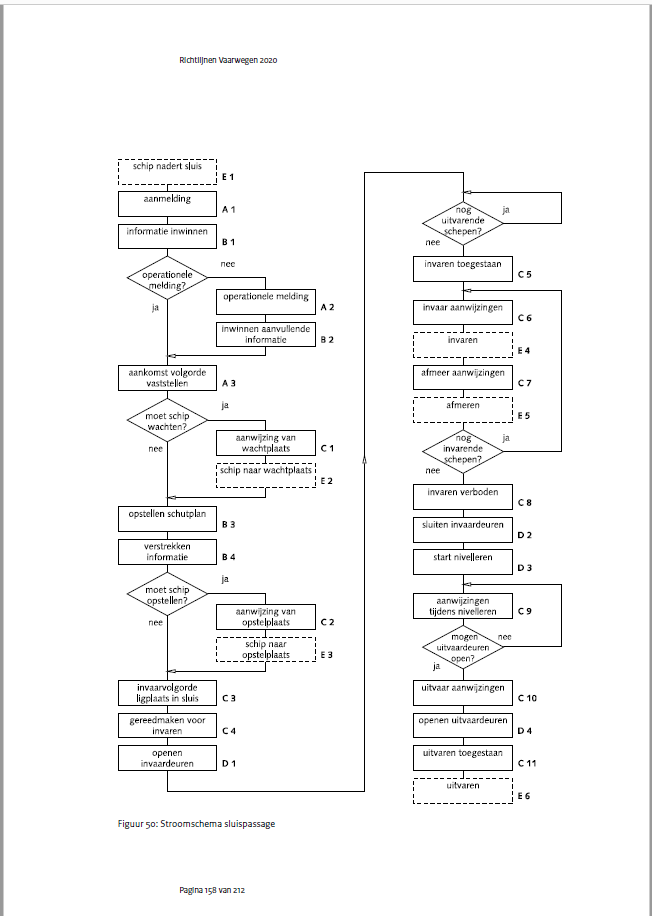
\includegraphics[width=8cm]{sluispassage.png} % also works with logo.pdf

 
	
	\section{Requirements elacitation}
	
	\subsection{Algemeen}
	
	Wat zijn requirements en specications?
	https://agilescrumgroup.nl/product-backlog/
	https://nl.wikipedia.org/wiki/Requirementsanalyse
	http://www.chilico.nl/artikelen/businessrequirements/business_en_functionelerequirements.html
	https://iir.nl/blog/goede-requirements-zijn-het-fundament-van-de-informatievoorziening/
	https://qualitybs.wordpress.com/2015/03/13/hoe-maak-je-een-user-requirement-specification-voor-operationele-systemen/
	https://www.bpmcompany.eu/in-hoeverre-zijn-requirements-en-specificaties-nuttig/
	https://www.reaco.nl/blog/wat-zijn-agile-requirements/
	Er bestaat ook een 6-variabelen model. . .Wat is dat?
	https://www.uni-due.de/imperia/md/content/swe/papers/icsoft16a.pdf
	Wat voor soorten requirements zijn er zoal te vinden?
	Hoe verkrijgt men requirements?
	Wat voor requirement elicitation technieken zijn er zoal?
	Wat is het verschil tussen functionele en niet-functionele
	requirements?
	Wat verstaat men onder mode confusion?
	http://automation.forthillgroup.com/themes/mode-confusion
	https://www.linkedin.com/pulse/confusion-cockpit-understanding-human-performance-david-thompson/
	Wat verstaat men onder de automatiseringsparadox?
	
		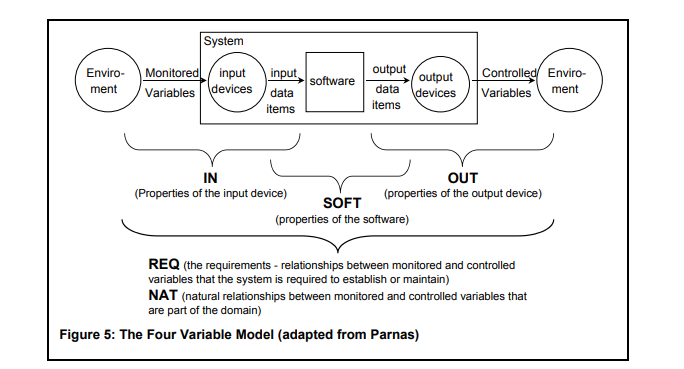
\includegraphics[width=8cm]{4varparnas.png}
		
				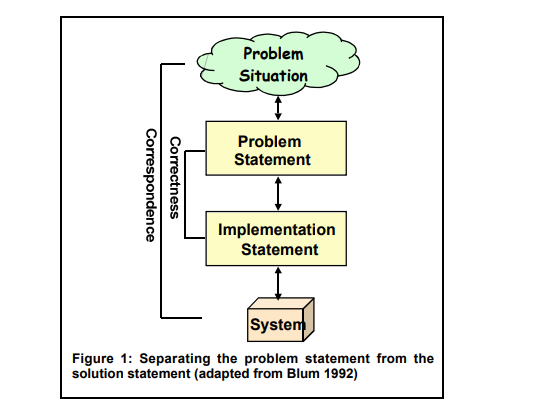
\includegraphics[width=8cm]{requirement.png}
		
			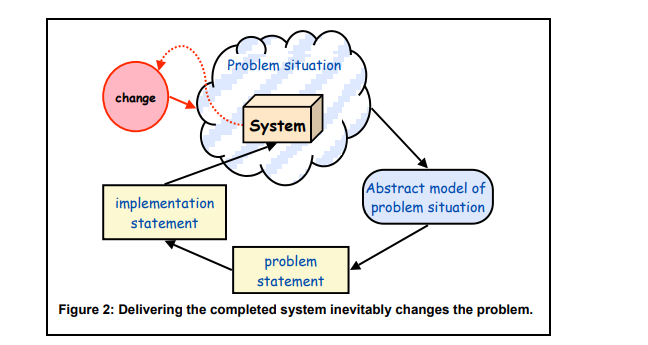
\includegraphics[width=8cm]{oplossing_easterbrook.png}
			
				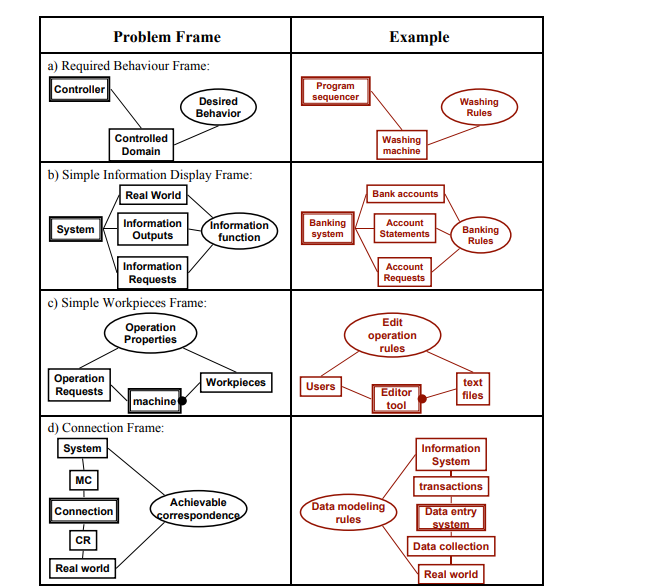
\includegraphics[width=8cm]{problemframejackson1997easterbrook.png}
				
			
					
						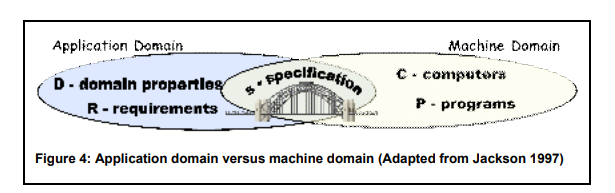
\includegraphics[width=8cm]{whatvshoe_easterbrook.png}
	Problem description vs slution description \\
	whatvs how \\
	application domain vs machine domain \\
	functional vs non-functional requirements \\
	systems engineering vs software engineering \\
	customers vs users \\
	ndicatieve vs optative descriptions \\
	verification vs validation \\
	capturing vs synthesisingrequirements \\
	
	\subsection{Conclusies uit rampenonderzoek van de groepsleden}
	
	
	\subsection{Requirements}
	Directe requirements van opdrachtgever:\\
	Na grondige analyse van het Nederlandse sluizenpark is gebleken dat renova-tie van een groot aantal sluizen noodzakelijk is.  Een eerste verkenning heeft onsgeleerd dat het gecombineerd renoveren en automatiseren van het Nederlandsesluizenpark een aanzienlijke verbetering kan opleveren t.a.v.:\\
	- veiligheid\\
	- efficientie\\
	- capaciteit\\
	- onderhoudskosten\\
	- duurzaamheid\\
	In het kader van het onlangs afgesloten klimaatakkoord heeft de Nederlandseoverheid  daarom  besloten  over te gaan tot een ingrijpende renovatie van dediverse sluizen die ons land rijk is. Op het ministerie van infrastructuur en waterstaat is helaas onvoldoende kennis van ict en systemen aanwezig om eenen ander uit te voeren. Wij vragen u een model (of een onderling samenhangend aantal modellen)aan  te leveren, opdat ontwerpen van verschillende, volledig geautomatiseerde sluizen in de toekomst gerealiseerd kunnen worden.\\\\
	Eigen inbreng van deze requirements:\\
	Wij gaan er van uit dat het volgende van ons verwacht wordt:\\
	Maak een model dat als template dient gebruikt te worden voor het automatiseren van verschillende soorten sluizen. Verder moeten overwegingen gemaakt worden die goed onderbouwd zijn.\\\\ Aangezien er van ons alleen een model verwacht wordt, zullen wij ons geheel focussen op de fundamentele werking van de sluis en hierbij zullen wij ons dus niet bezig  houden met fysieke eisen zoals veiligheidshekjes en borden. Onze focus ligt geheel op de werking van de sluis; elke state waar de sluis zich in mag bevinden en welke beslissingen de sluis moet maken op basis van bestaande protocols en benoemde eisen. \\\\
	Deze requirements zullen hieronder uitgewerkt worden, per sluisonderdeel, deze bestaande uit de sluisdeuren, de sloplichten, de waterpomp en de boten.\\
	
	
	\subsection{Specificaties}
	Vanuit deze requiremenst kunnen verdere specificaties opgesteld worden.
	
	Even ter duidelijkheid: een requirement beschrijft wat een programma moet doen, en een specificatie beschrijft hoe men van plan is om deze requirements te realiseren.//
	Voorbeeld:// Requirement is dat de sluis meerdere boten moet kunnen verwerken; de specificatie zou hier zijn fdat de sluis minstens twee keer zo groot moet zijn dan de grootste boot die door de sluis kan.
	
		
	moet de intitial state altijd in een loop zitten in uppaal?
	wat zijn urgent channels?
	rampen? er staat wel iets in de planning maar kan geen lessen of verdere documentatie of requirements terug vinden?	
	
	
	gesprek wessel:
	main controller slim dat direction een bool is. 
	pomp is te slim, zoiu alleen maar aan of uit moeten gaan, of nog weg en in pompen maar meer niet. niets met waterlevel en aantal schepen.
	schip: niet doen. als een schip zich aanmeld, dan gebeuren er dingen, maar gaat hij naar binnen? je weet niet wat dat schip gaat doen want menselijk gedrag. beter niet het schip uitgebreid maken, maar eerder de sluis. te veel aannames.
	
	wessel model: alleen als wachtrij vol zit, doet de sluis iets.
	deur heeft een parameter zodat er meerdere deuren in de simulator neergezet kunnnen worden. ook bij wachtrij.
	
	stoplichen kunnen er wel in maar als je simpeler wilt, gaan die als eerste weg.
	zes variabelen model is voorgesteld maar niet goed op gereageerd. alleen er van af weten is genoeg.
	rampen alleen voor persoonlijk verslag
	
	\subsubsection{Aannames}
	
		De meeste sluizen die zich in Nederland bevinden zijn schutsluizen; deze sluizen zijn bedoeld om boten, zowel vrachtschepen als pleziervaart afhangend van de locatie van de sluis, te verwerken. Om deze reden gaan wij deze dus ook verwerken in ons model. Mocht een sluis niet bedoeld zijn om boten te verwerken, dan zou dit model alsnog toegepast kunnen worden opp desbetreffende sluis.
	Boten worden toegevoed aan de queue. Hoe dit gebeurt, dat ligt aan de specifieke sluis.  Sinds wij een template maken, hoeven wij geen rekening te hounden met hoe de schepen in de queue komen. Het enige wat wij hoeven te doen, is de data verwerken.
	
	Overige einsen op basis van eigen inbreng:\\
	
		\subsection{Formele specificaties}
	
	\paragraph{Safety}
	Safety Properties are used to verify that something
	bad will never happen. Dit kan worden gespecificeerd met de volgende vergelijking
	
	
	
	\square ( a_0 \implies (( \lnot a_2 \wedge \lnot a_3 ) \mathcal{U} a_1 ) \vee ( \lnot a_2 \wedge \lnot a_3 )) \\
	
	
 
 
		\forall x \, (P(x) \to Q(x)) & premise \\
		\forall x \, P(x) & premise \\\hspace*{-30pt} \\
 
		 
			P(x_0) & $\forall x \, \mathrm{e}$ 2 \\
			Q(x_0) & $\to \mathrm{e}$ 3, 4 \\
 
		\forall x \, Q(x) & $\forall x \, \mathrm{i}$ 3--5 \\
 
	
	
	
 
	
	
	\{a,b\} or \set†{a,b} \\
	\langle a,b \rangle or \gens†{a,b} \\
	
	
	f \colon A \to B \\

	f \circ g \\
	x \mapsto f(x) \\
	
	\begin{align*}
		f \colon \mathbb{R} &\to \mathbb{R} \\
		x &\mapsto x^2
	\end{align*}
	
	
	\paragraph{Reachability}
	Reachability properties are used to check whether
	a given state formula can be satisfied by some
	reachable state.
	
	\paragraph{Liveliness}
	Liveness properties are used to verify that
	something eventually will hold
	\paragraph{Security}
	
	\paragraph{Performance}
	
	Er is geen deadlock
	

	
	
	
	\newpage
	\section{Formeel model gerealiseerd in Uppaal}
	
	\subsection{Algemeen}
	
\subsection{Formal specification}
	Sommige safety en reachability requirements die gespecificeerd moeten worden zijn hieronder aangegeven.
	De deur mag alleen  geopend zijn als er een schip wil in-/uitvaren.
	De stoplicht mag alleen op groen staan als de deuren zijn geopend.
	De pomp mag alleen worden aangezet als alle sluisdeuren dicht zijn, de stoplichten op rood.
	Een schip bereikt de finished state alleen als de positie van de final state verschilt met de positie van de initial state.
	Er is geen deadlock formatie in het systeem.
	Het monitoring mechanisme van het systeem werkt als volgd:
	Op geen enkel moment, positie hoog of laag zijn de hoogte en laagte sensore 0 of 1 tegelijkertijd.
	Op geen enkel moment, positie hoog of laag zijn aan weerszijnde de sluisdeuren open en stoplichten op groen.
	
		\subsection{Maincontroller}
	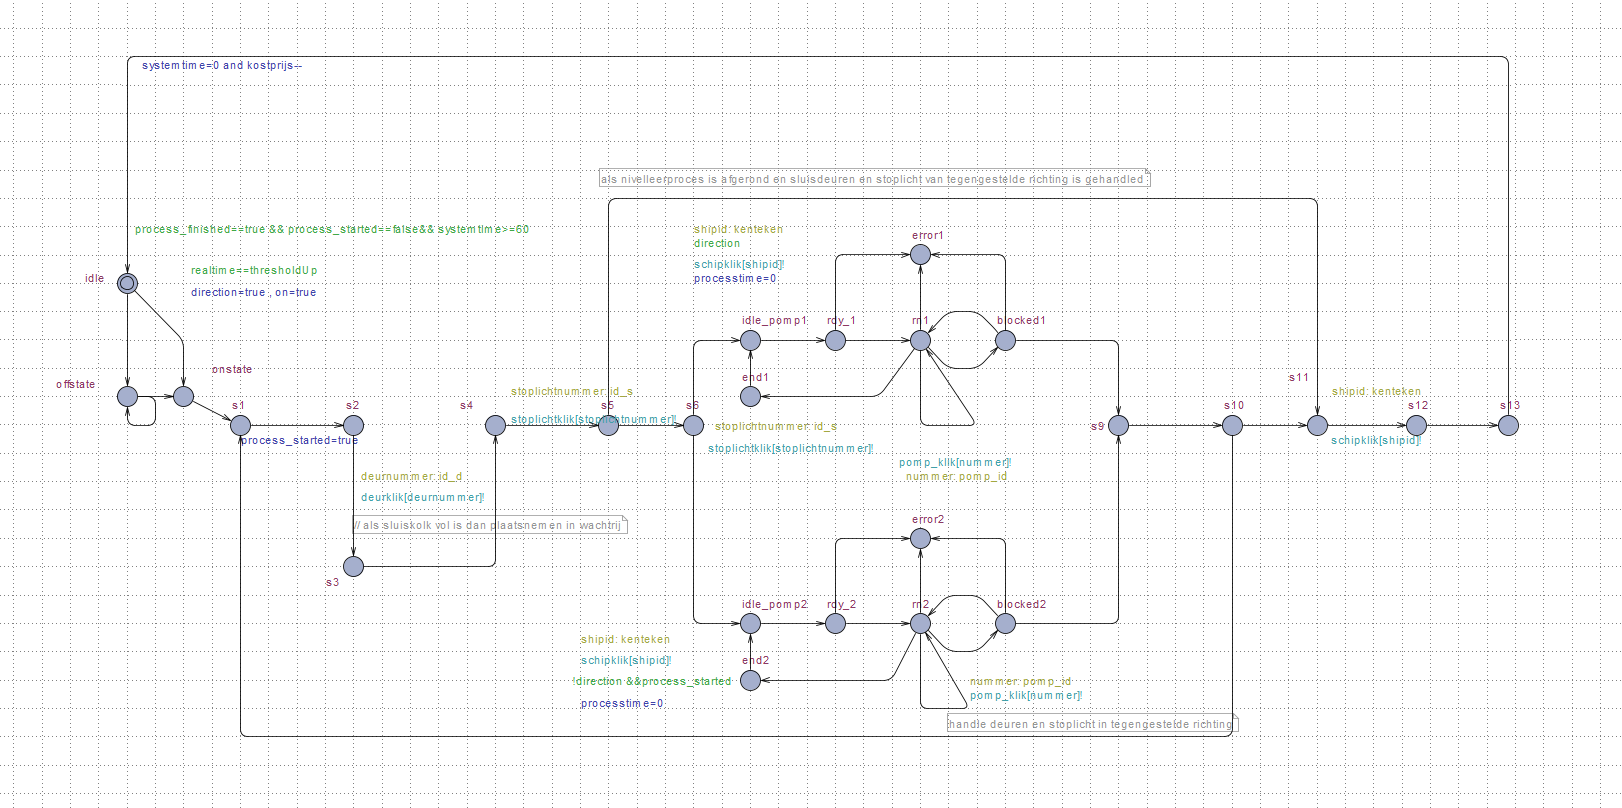
\includegraphics[width=8cm]{main.png} % also works with logo.pdf
	\subsection{Schip}
	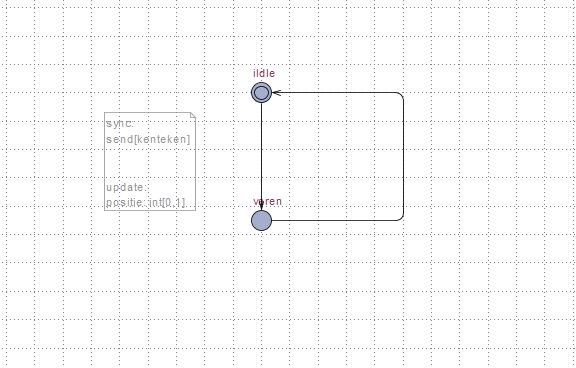
\includegraphics[width=8cm]{schip.png} % also works with logo.pdf
	\subsection{Sluiskolk}
	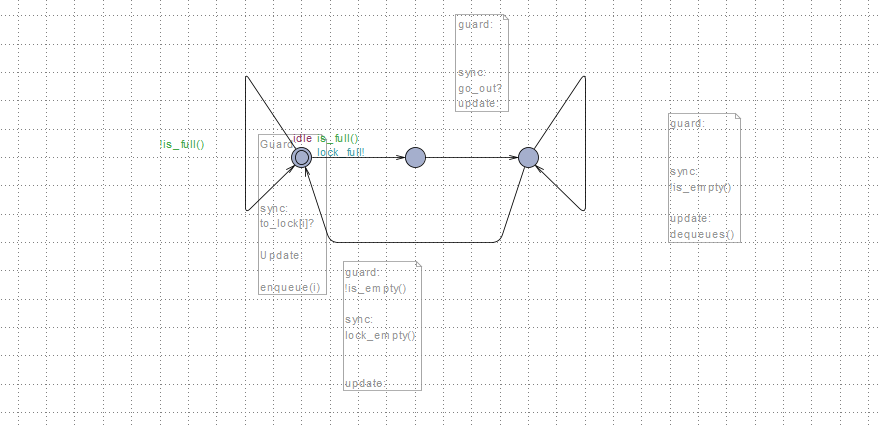
\includegraphics[width=8cm]{sluiskolk.png} % also works with logo.pdf
	\subsection{Stoplicht}
	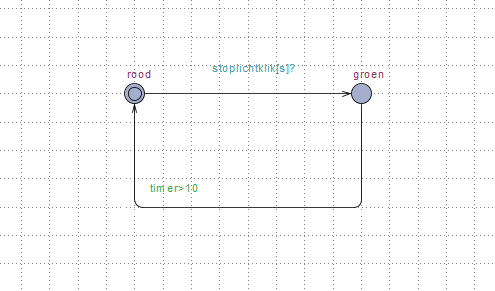
\includegraphics[width=8cm]{stoplicht.png} % also works with logo.pdf
	\subsection{Deur}	
	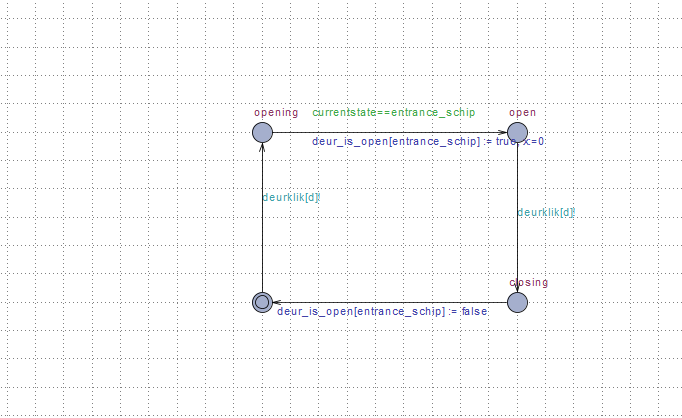
\includegraphics[width=8cm]{deur.png} % also works with logo.pdf
	\subsection{pomp}	
	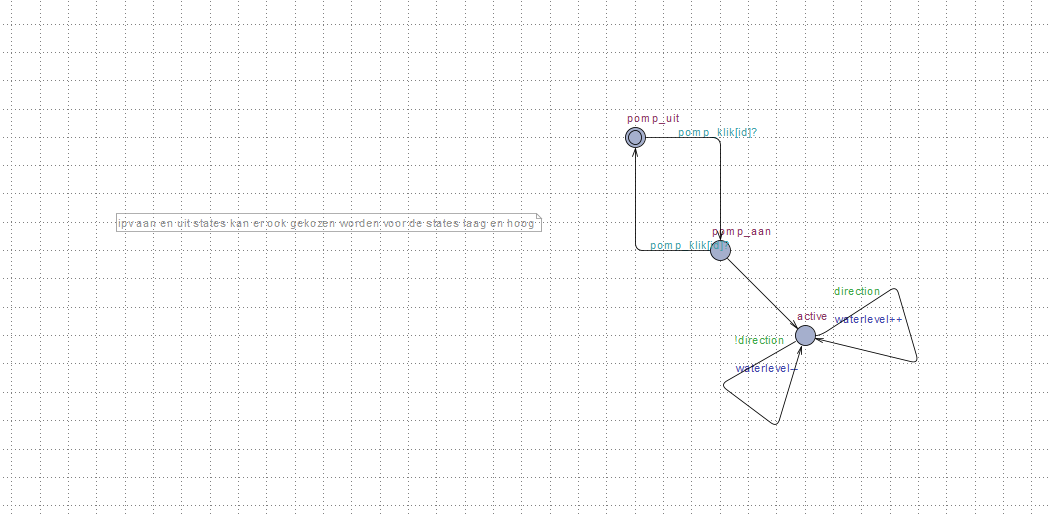
\includegraphics[width=8cm]{pomp.png} % also works with logo.pdf
	
	 

	 
	
	
	

	
	\subsection{De formele verificatie aan de hand van een Kripke structuur}
	De safety en reachability requirements die formeel zijn gespecificeerd   worden in Uppaal geverifieerd met de A en E state formule. Deze zijn als volgd:
	A[] not maincontroller.rd1 imply
	A[] maincontroller.rd1 imply
	A[] not deadlock imply
	E<> maincontroller.rd1 imply
	E<> maincontroller.s7
	E<> maincontroller.s7d


 
 
 
 Voor het modelleren van een systeemhebben we nodig:\\
 alle states van het systeem.We stoppen dezein een verzameling \\
 S: de verzamleing van alle states van een systeem
 Elke individuele state noemen we s_{0}, s_{1},...s_{n} \\
 Ons model is een tupelmet daarin de verzameling states: M(S)
 
 
 De transities tussen states vormen een relatie
 R $\subseteq$S xS
 
 De systemen die wij modelleren zijn reactief:Systemenkunnen eindeloos rondjes lopen door een aantal toestanden. \\
 Belangrijk gevolg: Voor elke state s \inS geldt dat er een state s' bestaat zodanig dat geldt R(s,s') \\
 Elke state heeft een uitgaande transities.
 Een transitierelatie, waarin elke stateeen uitgaande transitie heeft noemt men totaal. \\
 Alle transitierelatiesin de  systemen die wij modelleren zijn totaal.
 
 Om uitspraken te kunnen doen over ons systeem gebruiken we: \\
 Een verzamelingatomaire poposities (AP): proposities die niet verder op te delen zijnin kleinere/kortere proposities. \\
 Een labeling functie: L
 De labeling functieis een functie dieelke state "labeled"met een verrzameling atomaire propostities die waar zijn in die state: \\
   L= S \to   ~ $2^{AP}$  \\
 

 
 
 \paragraph{Model checking Temporal logics} \\
 M, s \models p $\Leftrightarrow$ p \in L(s) \\
 M, s \models \not f1 $\Leftrightarrow$ M, s \nvdash f1 \\
 M, s \models f1 \vee f2 $\Leftrightarrow$ M,s \models f1 or M,s \nvdash f2 \\
 M, s \models f1 \wedge f2 $\Leftrightarrow$  M,s \models f1 and M,s \nvdash f2 \\
 M, s \models \mathrm{E} g_{1} $\Leftrightarrow$ there is a path \pi  from ~  s ~   such ~  that  ~ M, \pi \models g1 \\
 M, s \models p $\Leftrightarrow$ for every path \pi  ~ starting from s, M, \pi \models g1 \\
 M, s \models p $\Leftrightarrow$ s is the first state of \piand M, s \models f1 \\
 M, s \models \not g_{1} $\Leftrightarrow$ M, \pi  \nvdash g1\\
 M, s \models p $\Leftrightarrow$  M, \pi  \models g1  or  M, \pi  M, \pi  \models g2\\
 M, s \models p $\Leftrightarrow$ M, \pi  \models g1  and  M, \pi  M, \pi  \models g2 \\
 M, s \models p $\Leftrightarrow$ M, $\pi^{1}$ \models g1 \\
 M, s \models p $\Leftrightarrow$ there exists a k \ge 0, such that M, $\pi^{k}$  \models g1\\
 M, s \models p $\Leftrightarrow$ for all i \ge 0,M,$\pi^{i}$ \models g1 \\
 M, s \models g1 \bugcup g2 $\Leftrightarrow$ there exists ak \ge 0 such that M, $\pi^{k}$ \models g2\\
 and for all 0 \le j < k, M,$\pi^{j}$ \models g1
 M, s \models p $\Leftrightarrow$ for all j \ge 0, if for every i < j,M,$\pi^{i}$ \nvdash g1 then M,$\pi^{j}$ \models g2\\
 
 
 
 

 
 Kripke structuur
  \mathbb{A}  bestaat uit  een 4-tuple M = \{ S ,  S_{0}  , \Re , L \} ~ met ~  daarin: \\
  S:  ~ de  ~ verzamelingvan ~  alle ~  states ~  in  ~ het ~  systeem \\
  S_{0} $\subseteq$ S: de verzameling van alle beginstates \\
  \Re $\subseteq$ \mathbb{S} x S: de transitierelatie \\
      L= S \to   ~ $2^{AP}$ ~ : de labels waarmee weiedere state labelen met atomaire propositiesdie waar zijn in die state\\

	\subsection{Tijd}
	
	\subsection{Guards en invarianten}
	
	\subsection{Deadlock}
	
	\subsection{Zeno gedrag}
	
 
	
	\subsection{Propositielogica}
	
	\subsection{Predicatenlogica}
	
	\subsection{Kwantoren}
	
	\subsection{Dualiteiten}
	
	\subsection{Proposities}
	
	\begin{itemize}
		\item  P1 Het is mogelijk dat de sluis van richting verandert.
		E<> !Main.Direction
		\item  P2 Het is mogelijk dat de sluispomp in een cyclus teveeel water heeft gepompt en dat er daardoor water weggepompt dan wel bijgekompt dient te worden
		E<> main.waterlevel
		\item  P3 Het is al binnen 100 ms mogelijk omte achterhalen aan welke kant de sluisdeuren  open moeten.
		\item  P4 Als de richting van een schip gelijk is aan N, dan is het waterlevel niet gelijk aan 1-5 of R
		\item  P5 De sluispomp is nooit in positie AAN, wanneer de sluisdeuren open zijn.
		\item  P6 In het geval dat er geen errors zijn (  in de stoplichten, sluisdeuren) and ideal (wachtrij) scenario,
		\item  a) dan is een cyclus gegarandeerd binnen 100 ms (including 100 ms) (undefined)
		\item  a') dan is een cyclus niet gegarandeerd binnen 100 ms
		\item  b)  dan is het onmogelijk om van beneden naar boven te varen, of andersom binnen 150 ms
		\item  b') dan is het mogelijk om van beneden naar boven te varen, of andersom binnen 150 ms
		\item  c) het is onmogelijk om van richting te veranderen in minder dan 400 ms als de pomp al op niveau x is
		\item  c') het is mogelijk om van richting te veranderen in minder dan 400 ms als de pomp al op niveau x is
		\item  P7 Als zich geen errors voordoen bij stoplicht en deur,maar de waterpomp uitvalt:
 
 
		
		
 
		\item  p12 Wanneer beide sluisdeuren in state gesloten zijn, dan is de pomp in zijn initiale state of 100 ms verwijderd van zijn initiele state
		\item  A[]
 
		\item  p14
		\item  a) Als de deur open is(ongeacht boven of beneden, dan bevind de sluispomp zich in een  predefined state (undefined)
		A[] (gate(0).open||gate(1).open) -> (main.pomp_idle || main.pomp2_idle)
		\item  b) Als de deur is gesloten dan bevind de maincontroller zich in een predefined state
		A[] gate.closed -> main.idle
		\item  p15
		\item  p16 If engine regulation is on torque, then the clutch is closed (undefined)
		A[](Engine.Torque imply Clutch.closed
		\item  p17Voor invaren geldt altijd: waterlevel, pomp uit, sluisdeuren open en stoplicht op groen
		A[] main.s5 -> main.waterlevel_laag && idle_pomp1 && gate(0).open && gate(1).open && (stoplight(0).green && stoplight(1).green || stoplight(2).green && stoplight(3).green )
		\item  p18 Als een schip van rechts binnen komt en sluisdeuren zijn dicht dan moet het stoplicht op rood, de pomnp in transitie van laag naar hoog en niet andersom
		A[] !main.direction -> forall (i:id_d) forall (j:id_s) gate(i).closed && stoplight.rood && main.rd_1
		p19 uitvarenden hebben voorang op invarenden
		
		\item  p20 Voor invarenden geldt pomp uit, sleusdeur open en stoplicht op groen
		A[] main.s6 -> gate(0).open && gate(1).open && stoplight(0).groen && stoplight(1).groen
		\item  p21 voor nivelleren geldt pomp is aan, sluisduren zijn doicht en het stoplicht is op rood
		A[] (main.rn1 || main.rn2) -> forall (i:id_d) forall(j:id_s )gate(i).closed stoplight(j).rood
		\item  p22 Als een schip vertrekt dan zijn altijd, sleusdeuren open, waterlevel gereed op niveau 5 of 0 en stoplicht direct op groen
		A[] main.s12 ->
		\item  p23 urgent locations; het is niet mogelijk om hier te wachten
		\item  p24 urgent syn; een synchronisatie moet direct worden uitgevoerd als de guards geldig zijn
		\item  p25 als een schip binnen is, en er zijn wachtende schepen, dan moet het stoplicht via oranje naar rood
		A[]
		\item  p26 committed; als deze staat actief is dan wordt de eerst volgende transitie uitaande van deze state
		\item  p27 als een schjip binnen vaart mnoiet hij ook eft binnen zijn en niet binnenvaren, dit geldt ook voor p28 sluisdeuren en pompen dus deze zijn committed.
		A[]
		\item  p28 Een schip komt aanvaren en geeft een signaal aan de sluis. 
		A[]	
		\item  p29 Indien er meer dan twee schepen in de sluis zitten dan wordt het ship geplaats in de wachrij. 
		A[]  Queue.list[N-1] == 2 -> (Sluiskolk.list[N]==1 ||Sluiskolk.list[N]==2)
		\item  p30 Een schip kan pas naar binnenrijden als de sluisdeuren open zijn, het stoplicht is op groen er er zijn minder dan 2 schepen in de sluis. 	
		A[]  main.s6 && schip.varen ->  Queue.list[N-1] <2
		\item  p32 Eenmaal in de sluis zal het schip moeten wachten op de sluis en de pomp. 	
		A[] Queue.list[N-1] == 2 
		\item  p33 Een schip mag alleen uitvaren als de pomp klaar is, de sleusdeuren open. 
		A[] schip.varen && main.s12 || main.s13 -> (!main.rn1 && !main.rn2)
		\item  p34 Een sluis ontvang een aankomst signaal van een schip en bestuurt de sluisdeuren en de pomp. 
		A[]
		\item  p35 De sensor is een onderdeel van de sluis en ontvangt signalen van naderende schepen. 
		A[]
		\item  p36 De sleusdeur voor boven en beneden kunnen beiden open en dicht. De sluisdeur wordt aangestuurd door de sluis. 
		A[]
		\item  p37 Een pomp begint met pompen bij een signaal van de sluis. Een sluis op zijn beurt geeft alleen een signaal aan de pomp als de sleudeuren dichtzijn
		A[] pomp.pomp_active -> main.s6 && forall(i:id_d) gate(i).closed
		\item  p38 Geen deadlock
		\item  p39 Voor geen enkel pad geldt dat als  de deuren gesloten zijn volgens de kluis dat er een deur openstaat om een schip naar buiten te laten.
		A[] not forall(i:id_d) gate.closed ->(main.s12||main.s13)
		\item  p40 Voor alle paden geld dat als een sluis aan het voorbereiden is, dan zijn alle deuren dcht.
		A[] main.s6 -> forall(gate(0).closed
		\item   p41 Voor alle paden geld dat als een deur dicht is het aantal schepen in de kade gelijk is aan nul	
		A[]
		p42 Voor geen enkel pad geld dat als het binnenstoplicht op groen staat dat het niet toegestaan in naar binnen te varen
		E<> stoplight(2).groen || stoploght(3).groen -> main.s6
		\item  p43 Voor alle paden geldt dat de globale tijd langer is dan 30 tijdseenheden
		A[] main.s13-> main.processtime>30
		\item  p44 Er is een pad waarvoor geld dat als een schip wilt stoppen dat er meer dan 5 schepen in de sluis zitten.
		E<>
		\item p45 Voor alle paden geldt als schip vrtrekt is sluisdeur dicht
		A[] 
		\item  p46 Voor alle paden geldt als stoplicht op rood sluisdeuren dicht en schip vertrokken dan is de nivelleermachine uit
		A[]
		\item  p47 Er is geen pad waarop een schip vertrekt vanuit de rechtersluisdeur en de linkersluisdeur is open en linkeruitaartstoplicht en linkeruitvaartsoplicht opgroen  en nibelleermachine is aan
		E<>
		\item  p48 Er is een pad waarvoor geldt dat linkerslsuisdeuren dicht zijn, rechtersluisdeuren dicht zijn rechteruitvaartstoplicht is rood en rechteruitvaartstoplicht is  rood terwijl eer geen schip in de sluis licht
		E<> 
		\item  p49 EEn stoplich staat altijd op groen als de deuren open staan en de pomp niet bezig is.
		A[] forall(i:id_s) stoplight.groen -> gate(0).open && gate(1).open && (main.pomp1_idle || main.pomp2_idle)
		\item  p50 In geen enkele staat van de sluis behalve tussen de lowergate en uppergate en uppergate en lowergate en de staten AtArrivalLow en AtEnteringHigh is de wachttijd langer dan 5 tijdseenheden
		A[] not
		\item  p51 Voor alle paden in een pomp geldt dat als water level lager is dan waterlaag pompwaterweg is altijd false
		A[] (main.waterlevel<waterlaag) -> (!pompwaterweg||pompwaterweg==false)
		\item  p52 Voor alle paden gelft dat als water level hoger is dan waterhoog dan is pompwater altjd false
		A[]
		\item  p53 Het zal nooit gebeuren dat een pomp water toevoegt als deuren open zjn, geen schip in sluis en stoplicht op groen
		A[] not main.rn1 || main.rn2 -> gate(0).open && gate(1).open && Queue.list[N-1] == 0 && ((stoplight(0).groen||stoplight(1).groen) ||(stoplight(3).groen &&stoplight(4).groen))
		\item  p54 Het kan gebeuren dat bij pompr het stoplicht op rood staat, het schip in de sluis en deur is dicht, en waterstand gelijk aan waterlaag
		E<> (main.blocked1 || main.blocked2) -> Queue.list[N-1] >0 && gate(0).closed && gate(1).closed && main.waterlevel==main.waterlevel_laag
		\item  p55 Er is een mogelijkheid  dat vanuit pomp get stoplicht op rood wordt gezet en waterlevel gelijk is aan waterlaag
		E<> main.rn1||main.rn2 -> gate(0).closed &&main.waterlevel==waterlaag
		\item  p56 Het kan voorkomen dat bij state pompaan het waterniveau gelijk is aan waterlaag
		E<> main.rn1||main.rn2 -> main.waterlevel== main.waterlaag
		\item  p57 Voor alle paden gelt dat er een mogelijkheid is dat deur is open/dicht en sluis nivelleert omhoog/omlaag
		A[] gate(0).open && ()main.direction ==0||main.direction==1)
		\item  p58 A[](1>0)
		

	\end{itemize} 
	
 
	
	\subsection{De computation tree}
	
\xymatrix@ur@!R=2pc{%
	*+<1pc>[o][F-]{q_0}  \ar@(l,l)[]^<<<<{start} \ar@/^/[r]^0  \ar@/_/[d]_1 
	& *+<1pc>[o][F-]{q_1} \ar@(ul,ur)[]^{0}  \ar@/^/[d]^1 \\
	*+<1pc>[o][F-]{q_2} \ar@(dr,dl)[]^{1} \ar@/_/[r]_0 
	& *+<1pc>[o][F=]{q_3} }
	
	\paragraph{Operator: AG}

	\paragraph{Operator: EG}
	

	Voor alle paden geldt dat het  waterlevel lager is dan het  niveau van de kant. (???)
	Voor alle paden geldt dat een pomp alleen werkzaam is als alle sluisdeuren dicht zijn.
	Vpoor alle paden geldt dat het aantal schepen in de sluis maximaal 2 is.
	Voor alle paden  geldt dat een schip nooit langer dan 30 seconden in een sluiskolk zit zonder dat het waterpeil is aangepast.
	\paragraph{Operator: EG}
	Er bestaat op elk pad een 

	\paragraph{Operator: AF}
	
	\paragraph{Operator: EF}
	Er is een mogelijkheid dat twee schepen in de sluis een verschillende uitvaarrichting hebben. (Hoe?)
	\paragraph{Operator: AX}

	
	\paragraph{Operator: EX}
	
	\paragraph{Operator: p U q}
	
	\paragraph{Operator: p R q}
	

	Voor alle paden geldt dat een schip alleen kan invaren als de sluisdeur aan de andere zijde is gesloten.
	\paragraph{Operator: EX}
	Er bestaat geen situatie waar een pomp actief is terwijl er een sluisdeur open staat
	\paragraph{Operator: p U q}
	Vanaf aankomst tot uitvaren is de clocktijd lager dan 30 tijdseenheden 
	\paragraph{Operator: p R q}
	Vanaf het invaren tot en met het uitvaren van een schip en geldig is x lager dan 15 tijdseenheden????
	vanaf aanvaren staat een schip maximaal 40 tijdseenheden in de wahtrij.
 
\subsection{Analyse}


	 \VerbatimInput{data.txt}
	\newpage
		\section{Conclusie}
		LIn this paper, we presented the case study of intelligent
		water level monitoring system. Different safety and
		reachability requirements of the system are specified,
		modelled and verified in the UPPAAL model checking
		tool.Also bugs in the requirements specifications were
		reported after counterexample analysis. Here failure in the
		sensors and timers are regarded as changes in the
		environment. Formal verification process validates the
		adaptive behavior of the system in defined changing
		environments. However, there is wide scope for defining
		various unaccounted changes in the environment and add
		additional functionality to the present system so that it
		will adapt to those changes.
		
		
			\newpage
		\section{Discussie}
		Conclusions
		It should always emphasize the key points presented in the article.
		It replies the research problem described in the introduction section. Discuss the inferences of the outcome, interpretations by the writer and identify the unsolved questions. 
		
		Summarise and draw the conclusions in present tense. It has 5% to 10% length of the core text
		Acknowledgement
		Acknowledge the people who have contributed in searching, structuring and writing of literature. Include full names of individuals who assisted the project to get results. Mention the name of the funding group and program. 
		Appreciate funding organisation/s.
		
		
		
		Conclusion
		In this paper, general guidelines and importance of review 
		article were discussed. After reviewing the literature it was found that the review article should follow the guidelines to make the article best and comprehensive. It is concluded that every section of review has its own importance.
		
		
		\subsection{Conclusie Galvin}
		
		Because of the lack of __ we decided to not investigate __
		One concern about the findings of __ was that __
		Because of this potential limitation, we treat __
		The limitations of the present studies naturally include __
		Regarding the limitations of __, it could be argued that __
		Another limitation of this __
		This limitation is apparent in many __
		Another limitation in __ involves the issue of __
		The main limitation is the lack of __
		One limitation is found in this case.
		One limitation of these methods however is that they __
		It presents some limitations such as __
		Although widely accepted, it suffers from some limitations due to __
		An apparent limitation of the method is __
		There are several limitations to this approach.
		One limitation of our implementation is that it is __
		A major source of limitation is due to  __
		The approach utilised suffers from the limitation that __
		The limitations are becoming clear __
		It suffers from the same limitations associated with a __
		
		https://www.ref-n-write.com/blog/research-paper-example-writing-results-discussion-section-academic-phrasebank-vocabulary/
		
		\subsection{Conclusie Tygo}
		
		\subsection{Conclusie Koosha}
		
		\subsection{Challenges ahead}
		
		
		
			\newpage
		\section{Eindverantwoording}
		many thanks to all of you. Zonder jullie was dit nooit gelukt.
		
		\section{Bijlageoverzicht}
		
		
		\newpage
		\section{General considerations.}
		
		\section{Acknowledgements}
		
		\section{Data availability statement}
		
		\section{Abbreviations}
		
		\section{	Financial support and sponsorship}
		
		
		\appendix
		
		
		\section{ List of requirements }
		
		\section{ Schematics }
		
		\section{ Bill of Material }
		
		\section{ Use-Case flow charts}
		
		\section{Competences}
		
		\section{ Gannt planning }
		
		\section{Authors' contributions}
		
		\section{Data availability statement}
		
		\section{Declarations}
		
		\section{Footnotes}
		
		\section{Contributor Information}
		
		 
		
	
		\newpage
		\section{Conflicts of interest}
		
		
		
		
		
	\bibliography{references}
	\bibliographystyle{plain}
	
	\newpage
	\section{Hoe schrijf ik een wetenschappelijk artikel}
	Prologue‘A well begun is half done’ Author must thinkbefore hand, about “How to write?” “What to write?” and“Where to submit?”. Having affirmed all of the above,with the data of a well conducted and concluded researchproject in hand, author must think of a “clear message”intended to be given through his write up. A good measureof success is the conclusions drawn from the study, if canbe written in one meaningful sentence.The others considerations to be decided priorly are
	i) What is the best format of presentation of the researchdone? eg: as  original article, review, case report, orcorrespondence,? because format is different fordifferent type of articles.
	ii) Target audience for the publication and whichjournal?: Aspiring authors will improve their chanceof acceptance if they choose an appropriate journalfor their topic and adhere to conventional rules. Thereason why this decision must be taken in the earlyphases is that from the first draft, the paper must bewritten in the style and format of the specific, journaltargeting particular group of audience.
	iii) A thorough literature search is quite essential : 
	a) toidentify the knowledge gaps in the existing informationand the proposed paper may be aimed to fill themup. 
	b) to avoid duplication if the same message orproject has been published already.  Most journalsdo not wish to consider for publication a paper orwork that has already been reported in a publishedpaper.
	iv) Other matters related to authorship, ethical,  andstatistical clearance may be obtained well in advance.
	
	
	I)  Title1) Title should correctly represent the content andbreadth of the study reported and should  not bemisleading.For example “comparative evaluation of  Propofol– Ketamine and Propofol Fentanyl  in minorSurgery”. On reading the title, we can not know thecontent and breadth of the study; whether dosage,duration, efficiency, and sequalae, of two group arestudied or not whether they are studied as onlyinduction agents or as sole anaesthetic agents; whatgroup of patients? None of the information can behad from this title.
	
	2) It should be clear, concise, and informative. Itshould contain keywords, that capture attention ofthe reader. No abbreviations are used in the title.The decision to read an article often  rests on theappeal of its title.      A More appropriate title could be –“Comparativeevaluation of efficiency of Propofol – Ketamineand Propofol – Fentanyl combination as soleanaesthetic agents in patients undergoing minorambulatory  gynecological operations”.
	II) Author
	3) Designation,  degree, affiliation and address ofauthors are to be clearly indicated, with additionaldetails like telephone   number, email  address ofthe corresponding author.
	III) Abstract  & Keywords
	4) Abstract should cover each and every componentof, the study in 150 words for ‘unstructured’ abstractsand 250  words for ‘structured’  abstracts. It shouldstate the purpose of the study or investigation,basic procedures, (selection of study subjects,methodology, main findings, statistical significance),the principal conclusion and implications.
	5) The abstract should contain precise information andshould not contain abbreviations.
	6) The implications and benefits should commensuratewith the results obtained, and are to be highlighted.
	7) Key words (or short phrases) 3 to 10, should belisted covering all the aspects of the study. Usepreferably the terms listed as Medical subjectheadings (MESH) in Index Medicus (Medline)
	IV) Introduction and Review of Literature
	8) The goal or purpose of the study is clearly stated.The introduction should contain detailed informationabout the problem being studied,   and about thespecific research question/hypothesis.
	9) Four or five pertinent publications related to theproblem should be presented and critiqued.  Nodata or conclusions are to be reported.
	10) Do not review the literature  extensively.
	11) The pertinence of the study is  presented,  inrelation to the current theories and methodsassociated with the problem. The existing gaps  inthe knowledge or conflicting data is to behighlighted.
	12) A general overview of the study is presented. Overview serves as   organiser for the sections to followto the reader.
	
	
	V) Material and Method
	13) The selection of the subjects for the study has to bedescribed clearly. Inclusion and exclusion criteriaare to be mentioned with method of allocation togroups.
	14) The research design is to be described in detail.Research design is the plan that is chosen to answerthe research question.  The methods, apparatus  andprocedures are to be identified  in sufficient detail toallow other workers to reproduce the results, ifnecessary.
	15) Give references of  all the methods used in the studyincluding statistical methods.
	16) Identify precisely all drugs and chemicals used,including generic names, doses and routes ofadministration.
	17) Methods of elimination of errors viz blinding,introduction of control group and placebo,randomization etc are to be mentioned distinctly.
	18) The measurement instrument including itspsychometric qualities is described clearly.  Thepsychometric qualities include validity, reliability,objectivity  and precision.  An example of theinstrument should be gives in the text or in anappendix.For example in the above mentioned study, if ‘homereadiness’ is intended to be studied, the ‘PostAnaesthetic Discharge scoring system’ (PADS)utilised in the study has to be a reliable, and anaccepted one for its objectivity and precision.
	19) The data collection procedure is to be clearlydescribed.
	20) The setting in which the study took place is described.This information is useful to the reader in decidingwhether results can be applied to his/her setting.
	21) The data analysis procedures are stated in preciseterms.
	
	VI) Results
	22) Present your results in logical sequence  in the text,tables and illustrations.  Do not repeat in the text allthe data, in the tables or illustrations.
	23) Emphasize or summarise important observations.Results  section should contain only  actuals, and noopinions.
	24) All the patients included in the study should beaccounted for. There should not be any hesitation inreporting any negative or unexpected result
	
	VII) Discussion & Conclusion
	25) The discussion should cover all the debatable  aspectsof the study. The discussion  can go beyond theresults obtained and can cover methodological andthe critical issues. The discussion should not bemisused as a platform to state opinions. Readersshould not be side tracked in to another topic.
	26) Relate the observations to the other relevant studies.Bring out similarities and conflicts.
	27) The new and important aspects of the study and theconclusions drawn are to be emphasized.  Theimplications  of the findings and their limitations areto be discussed.For example if you find that  Propofol – kelaminecombination fared well except that there was‘excitatory phenomenon’ of Ketamine observed inthese group of patients, this limitation has to bementioned without fail.
	28) Scope  and need for future additional research is tobe  discussed.
	29) Link conclusions with goals of the study but avoidunqualified statements and conclusions not supportedby your data.
	30) State new hypothesis when warranted .Recommendations when appropriate may be included.For eg Propofol does not have any effect on excitatoryphenomenon associated with Ketamine.
	31) The conclusions and practical outcomes of the studyshould commensurate with the design used and resultsobtained.  The conclusions and recommendationsmade should not go beyond the limits of the studyconducted i.e. should not over generalize the designand sample used.Suppose the haemodynamics were stable in Ketamine-Propofol group as compared to Propofol – Fentanylgroup, one should not generative that the combinationis recommended for patients with cardiovasculardiseases
	
	
	
	Viii) References
	32) This is the most disturbing aspect amongst the Indianpublications. It is a wrong notion amongst Indianauthors that providing a long list of referencesincreases the validity (of their article) which is wrong.References are to be written correctly with due care.Correct abbreviated, accepted names, of the journalsto be mentioned. The number of references should
	be reasonable (neither too many nor too few); Somejournals specify the number of references to beincluded in a particular type of study.
	33) Avoid using ‘abstracts’ as references.  The referencesmust be verified by the author against the originaldocuments.
	34) The references are presented according to standardrules of publication as specified by a particularjournal. for eg, whether Vancour style or Harwardstyle is followed.General  Considerations
	35) The various sections of the paper are clearlyidentifiable and appropriate. The content of eachsection should correspond to the subtitle used, forinstance, there is no ‘Discussion’ in the ‘Results’section. The transition from one section to nextshould be easy to follow.
	36) The terminology has to be uniform through out thepaper. For eg.  abbreviations  should be consistentand units of measurements should be the same inthe text as in tables.
	37) The writing style has to be clear and pleasant.  Thereshould not be spelling mistakes. Special care isneeded in following British Vs American spellings.Text is, generally written is passive voice.  Uniform‘tense’ has to be used.
	38) Follow the instructions of the journal, you arewriting regarding tables, graphs illustrations, thetext matter, type of  manuscripts etc. to be used inthe article.
	39) Follow the ethical guidelines strictly as specifiedby ICMJE. If there is confusion as what is ethicaland what is non ethical and there is no ethicalcommittee to guide, ‘a self test’ may be employed.Ask yourself whether you will be conducting thesimilar study  on your kith and kin. If yes, goahead with your study.
	
	40)  All the direct and  indirect help in the study hasto be acknowledged, without fail.Editors and referees ……………………. but are busypeople whose humanitarian instincts should not be abused;and it is better for all concerned if authors try to submitpapers that are in good working order5 
	https://www.researchgate.net/publication/265059173_How_To_Write_A_Scientific_Article_For_A_Medical_Journal
\end{document}


